\chapter{\textbf{Sistemas lógicos formales: Lógica Temporal de Acciones}}
Este capítulo se adentra en los fundamentos matemáticos de una de las partes claves de este proyecto: el estudio y la evolución de la lógica formal, con la aplicación práctica a la corrección de sistemas concurrentes. La lógica, desde sus orígenes, ha tenido la aspiración de simbolizar y sistematizar el razonamiento humano. Esta simbolización emplea elementos del lenguaje humano, conocidos como \textit{sentencias}, que son declaraciones susceptibles de ser categorizadas como verdaderas o falsas. Se comienza por explorar los principios básicos de la lógica proposicional (\cite[Capítulo 8]{monk1976mathematical},\cite{garciaolmedo2018lprop} ),  la más elemental y fundamental para este fin. Sobre esta base, se desarrollan \textit{extensiones} que permiten abordar razonamientos más complejos. Un ejemplo notable es la lógica modal \cite{jansana2003logicamodal}, que introduce los conceptos de \textit{necesidad} y \textit{posibilidad}. Estos conceptos enriquecen el análisis lógico al permitir la exploración de diferentes mundos posibles y escenarios hipotéticos. La lógica modal sienta las bases para entender cómo ciertas proposiciones pueden ser necesariamente verdaderas o posiblemente verdaderas en diferentes contextos, lo que resulta crucial en el análisis de sistemas dinámicos y cambiantes.

El punto culminante de este capítulo es la Lógica Temporal de Acciones (\cite{lamport1994temporal},\cite{abadi1990axiomatization} ), conocida por sus siglas en inglés como TLA. Esta lógica se distingue por su capacidad para modelar y analizar secuencias de acciones en sistemas, considerando tanto su secuencia como su temporalidad. La relevancia de TLA, junto con la Lógica Temporal Lineal, radica en su aplicación fundamental para la verificación formal de propiedades en sistemas concurrentes, donde el orden temporal y las interacciones son cruciales. La implementación de estas lógicas facilita la descripción y verificación formal de especificaciones y propiedades a lo largo del tiempo, garantizando así el correcto funcionamiento y fiabilidad de los sistemas. Con esta metodología, después se pueden desarrollar o simular sistemas en un lenguaje de programación de manera más eficiente y segura, como es el caso de la solución informática realizada en este proyecto, descrita en posteriores capítulos.

\section{Conceptos básicos matemáticos}\label{section:concepts}
En esta sección se introducen algunos conceptos elementales previos necesarios para el estudio realizado en posteriores secciones del capítulo.

\subsection{Operaciones entre conjuntos}
\noindent
Se presentan algunas de las operaciones más básicas entre conjuntos:

\vspace{0.5cm}
\noindent
\textbf{Partes de un conjunto}

Sea $X$ un conjunto. Se define $\mathcal{P}(X)$ como el \textbf{conjunto de las partes de $X$}, cuyos elementos son todos los subconjuntos de $X$. Formalmente, $A \in \mathcal{P}(X)$ si y sólo si $A \subset X$.

\vspace{0.5cm}
\noindent
\textbf{Intersección}
\noindent
\newline
Sea $X$ conjunto y $A,B \in \mathcal{P}(X)$. Se define la \textbf{intersección} $A \cap B$ como:

\begin{align*}
    A \cap B := \lbrace x \in X : (x \in A) \hspace{0.1cm} y \hspace{0.1cm} (x \in B) \rbrace
\end{align*}

\vspace{0.5cm}
\noindent
\textbf{Producto cartesiano}
\noindent
\newline
Sea $X$ conjunto y $A,B \in \mathcal{P}(X)$. Se define el \textbf{producto cartesiano} $A \times B$ como:

\begin{align*}
    A \times B := \lbrace (a,b) : (a \in A) \hspace{0.1cm} y \hspace{0.1cm} (b \in B) \rbrace
\end{align*}

\subsection{Relaciones binarias}\label{subsection:binaryrel}
Sea $X$ un conjunto. Se denomina \textbf{relación binaria sobre $X$}, denotado por $R$, a un subconjunto de $X \times X$. Si dos elementos $x,y \in X$ están relacionados, se escribe como $(x,y) \in R$ ó $xRy$. Se distinguen diferentes tipos de relaciones binarias en función de sus propiedades:

\begin{itemize}
    \item \textbf{reflexiva} si $\forall x \in X, (x,x) \in R$.
    \item \textbf{irreflexiva} si $\forall x \in X, (x,x) \not \in R$.
    \item \textbf{simétrica} si $x,y \in X, (x,y) \in R$ implica que $(y,x) \in R$.
    \item \textbf{antisimétrica} si $\forall x,y \in X : (x,y) \in R$ y además $(y,x) \in R$, implica que $x = y$.
    \item \textbf{transitiva} si $\forall x,y,z \in X, (x,y),(y,z) \in R$, entonces $(x,z) \in R$.
    \item \textbf{serial} si $\forall x \in X, \exists y \in X : (x,y) \in R$.
    \item \textbf{euclidiana} si $\forall x,y,z \in X, (x,y),(x,z) \in R$, entonces $(y,z) \in R$.
    \item \textbf{de equivalencia} si $R$ es \textit{reflexiva, transitiva y simétrica}.
    \item \textbf{total} si $\forall x,y \in X$, $(x,y) \in R$ ó $(y,x) \in R$.
\end{itemize}

\section{Fundamentos de la lógica proposicional}\label{section:lprop}
En esta sección, se revisan los principios fundamentales de la lógica proposicional (\cite[Capítulo 8]{monk1976mathematical},\cite{garciaolmedo2018lprop} ), explorando sus elementos sintácticos, su semántica, y algunos resultados importantes que serán de utilidad en secciones posteriores. Estudiar la lógica proposicional no sólo es crucial para entender las estructuras lógicas más avanzadas como la lógica modal (~\ref{section:lmodal} ) y la Lógica Temporal de Acciones (~\ref{section:TLA} ), sino que también es fundamental en diversas aplicaciones prácticas. En informática, por ejemplo, es la piedra angular en el diseño de circuitos digitales y en la formulación de algoritmos. Su simplicidad y rigor proporcionan el marco necesario para construir argumentos lógicos sólidos y para desarrollar sistemas complejos con precisión y claridad.


La lógica proposicional, como punto de partida en el estudio de las lógicas formales, establece la base para la comprensión y el desarrollo de sistemas lógicos más complejos. Esta lógica opera con unidades básicas del pensamiento conocidas como \textbf{proposiciones}. Estas proposiciones son \textbf{sentencias atómicas, indivisibles}, que pueden ser inequívocamente categorizadas como verdaderas o falsas, sin ambigüedad. También se dispone del uso de $\textbf{conectivas}$ u \textbf{operadores lógicos}, que son elementos que permiten conectar las proposiciones permitiendo expresar nociones lógicas como \textit{implicación}, \textit{no}, \textit{y}, \textit{o}, etc. Usar de manera combinada proposiciones con operadores lógicos permite construir sentencias más complejas, donde su veracidad puede ser \textit{inferida} a través de la veracidad o falsedad de sus componentes.



\subsection{El lenguaje proposicional}\label{subsection:lproplenguaje}
El lenguaje proposicional contiene los elementos con los que trabaja la lógica proposicional. Formalmente, un \textbf{lenguaje proposicional} $\mathcal{L}$ es una dupla $(O,P)$ tal que $O,P \neq \emptyset$ y $O \cap P = \emptyset$. Al conjunto $O$ se le llama ``conjunto de conectivas u operadores lógicos'', mientras que a $P$ se le denota por ``conjunto de proposiciones''. La unión de estos dos conjuntos incluyendo a los paréntesis $\lbrace (,) \rbrace$, $O \cup P \cup \lbrace (,) \rbrace$, es el ``conjunto de \textbf{símbolos}'' de $\mathcal{L}$. A los elementos de $P$ convendrá escribirlos con letras del abecedario minúsculas, incluyendo eventualmente subíndices: $a,b,c,a_0,a_1,a_2$, etc.

Esta definición formal de lenguaje permite definir con libertad el repertorio de operadores lógicos a utilizar, es decir, el conjunto $O$. Dependiendo de sus elementos, se tiene un lenguaje proposicional diferente. La lógica proposicional tradicional puede utilizar varios conjuntos de conectivas, aunque en este estudio se opta por utilizar estas cinco citadas a continuación:

\begin{itemize}
    \item $\land$ : conjunción.
    \item $\lor$ : disyunción.
    \item $\rightarrow$ : implicación.
    \item $\leftrightarrow$ : equivalencia o doble implicación.
    \item $\neg$ : negación.
\end{itemize}

En algunos libros como \cite[Capítulo 8]{monk1976mathematical} se utiliza un subconjunto reducido de las indicadas anteriormente, concretamente $\lbrace \neg, \rightarrow \rbrace$, usualmente referidas como conectivas primarias. El motivo es que el resto de las conectivas se pueden expresar en términos de éstas (véase ~\ref{subsubsection:lpropequivalency}). Por otra parte, si se incluyen operadores nuevos se está \textbf{extendiendo} la lógica proposicional, dando como lugar otras nuevas como las que se verán a lo largo de este capítulo. En definitiva, en lo que sigue para esta sección se considera $C = \lbrace \neg, \rightarrow, \land, \lor, \leftrightarrow \rbrace$ por mera comodidad.

\subsection{Expresiones y fórmulas}\label{subsection:lpropform}
Una vez determinados los elementos más básicos del lenguaje proposicional, lo que sigue es indicar cómo manipularlos formando otros elementos del lenguaje más complejos para así poder cumplir con el objetivo descrito de simbolizar el razonamiento humano. Siendo $\mathcal{L} = (O,P)$ un lenguaje proposicional, se entiende por \textbf{expresión} a una sucesión finita no vacía de sus símbolos. Se dice además que dos expresiones $A,B$ son idénticas si lo son símbolo a símbolo, y se escribe como $A \equiv B$. Ejemplos de expresiones son ``$a(\land bc \rightarrow d\neg$'' y ``$a \rightarrow (b \land c)$''. Sin embargo, el segundo ejemplo parece mantener una cierta ``coherencia'' o ``equilibrio'', motivando la distinción entre expresiones y \textit{fórmulas}. 

Se entiende por \textbf{fórmula bien formada} o simplemente \textbf{fórmula} de un lenguaje proposicional $\mathcal{L}$ a las expresiones de la forma:

\begin{itemize}
    \item $p$, con $p \in P$ (es decir, una proposición atómica), leyéndose como ``fórmula atómica''.
    \item si $\alpha,\beta$ son fórmulas:
    \begin{itemize}
        \item $(\alpha \rightarrow \beta)$, leyéndose como ``$\alpha$ implica $\beta$''.
        \item $(\alpha \lor \beta)$, leyéndose como ``$\alpha$ o $\beta$''.
        \item $(\alpha \land \beta)$, leyéndose como ``$\alpha$ y $\beta$''.
        \item $(\alpha \leftrightarrow \beta)$, leyéndose como ``$\alpha$ equivale a $\beta$''.
        \item $(\neg\alpha)$, leyéndose como ``no $\alpha$''.
    \end{itemize}
\end{itemize}

y se denota al conjunto de todas las fórmulas de $\mathcal{L}$ por $Form_{\mathcal{L}}$. Se conviene en decir que todo objeto que no haya sido obtenido a partir de las reglas anteriores, no pertenece a este conjunto. En otras palabras, no hay más fórmulas proposicionales a parte de las definidas. Se utilizarán letras del alfabeto griego para referirse a las fórmulas del lenguaje, también utilizando subíndices si se necesita: $\alpha,\beta,\gamma,\alpha_0,\alpha_1$, etc.

\noindent
Ejemplos de fórmulas proposicionales son las siguientes:
\begin{itemize}
    \item $\alpha_1 = p \lor q$
    \item $\alpha_2 = r$
    \item $\beta_1 = p$
    \item $\beta_2 = q \rightarrow r$

    \item $\gamma_1 = \alpha_1 \rightarrow \alpha_2 = p \lor q \rightarrow r$
    \item $\gamma_2 = \beta_1 \lor \beta_2 = p \lor q \rightarrow r$
\end{itemize}

La escritura de las fórmulas $\gamma_1$ y $\gamma_2$ es exactamente igual, y sin embargo, son dos fórmulas \textit{diferentes}. He aquí donde reside la importancia de considerar a los paréntesis como símbolos del lenguaje, para evitar este tipo de ambigüedades. \footnote{Al igual que ocurría con las conectivas, otros textos como \cite[Capítulo 8]{monk1976mathematical} emplean la notación polaca (también conocida como \textit{Polish notation}), que es una forma de escribir expresiones lógicas y matemáticas sin paréntesis. Esta notación contribuye a una distinción más clara entre el lenguaje formal, que en este caso prescinde de paréntesis, y un metalenguaje que los utiliza.} 

Por otro lado, a partir de la definición de fórmula del lenguaje proposicional queda claro que la obtención de una fórmula $\alpha$ se realiza a partir de fórmulas más sencillas mediante uso de conectivas. Dada $\alpha \in Form_{\mathcal{L}}$, se define el conjunto de \textbf{subfórmulas} de $\alpha$, $Sub(\alpha)$, como:

\begin{itemize}
    \item $Sub(\alpha) = \lbrace \alpha \rbrace$, si $\alpha \in P$.
    \item $Sub(\alpha) = \lbrace \alpha \rbrace \cup Sub(\alpha_1) \cup Sub(\alpha_2)$, si $\alpha = \alpha_1 \lor \alpha_2$.
    \item $Sub(\alpha) = \lbrace \alpha \rbrace \cup Sub(\alpha_1) \cup Sub(\alpha_2)$, si $\alpha = \alpha_1 \land \alpha_2$.
    \item $Sub(\alpha) = \lbrace \alpha \rbrace \cup Sub(\alpha_1) \cup Sub(\alpha_2)$, si $\alpha = \alpha_1 \rightarrow \alpha_2$.
    \item $Sub(\alpha) = \lbrace \alpha \rbrace \cup Sub(\alpha_1) \cup Sub(\alpha_2)$, si $\alpha = \alpha_1 \leftrightarrow \alpha_2$.
    \item $Sub(\alpha) = \lbrace \alpha \rbrace \cup Sub(\alpha_1)$, si $\alpha = \neg\alpha_1$.
\end{itemize}

Es decir, si $\alpha$ es una fórmula atómica, su única subfórmula es ella misma, mientras que si es una fórmula obtenida a partir de otras fórmulas más sencillas con el uso de una conectiva, éstas son subfórmulas de $\alpha$ (denominadas concretamente como \textbf{subfórmulas inmediatas}), así como todas las que han intervenido en la formación de cada subfórmula.

\subsubsection{El principio de lectura única}
Una observación importante con respecto a lo comentado en los ejemplos de fórmulas anteriores es que no hay que confundir el hecho de que dos fórmulas diferentes puedan tener una misma escritura con que, sea cual sea la fórmula $\alpha$ a considerar, sólo existe una única forma de escribirla, lo que se conoce como \textit{principio de lectura única}.

\begin{teorema}
    \textbf{Principio de lectura única}. Sea $\mathcal{L} = (O,P)$ un lenguaje proposicional y $Form_{\mathcal{L}}$ el conjunto de fórmulas proposicionales del lenguaje. Entonces:
    \begin{enumerate}[label=\Roman*.]
        \item Toda fórmula es de longitud positiva.
        \item Si $\phi \in Form_{\mathcal{L}}$, entonces o $\phi = p$ con $p \in P$, o $\phi = \neg \alpha$ con $\alpha \in Form_{\mathcal{L}}$, o $\phi = \alpha \land \beta$, o $\phi = \alpha \lor \beta$, $\phi = \alpha \rightarrow \beta$, $\phi = \alpha \leftrightarrow \beta$, con $\alpha,\beta \in Form_{\mathcal{L}}$.
        \item Si $\phi = \langle \phi_0,\ldots,\phi_{m-1} \rangle \in Form_{\mathcal{L}}$ y además $i < m-1$, entonces $\langle \phi_0,\ldots,\phi_{i} \rangle \not \in Form_{\mathcal{L}}$.
        \item En (II), las posibilidades mencionadas son mutuamente excluyentes, y las fórmulas $\alpha,\beta$ están unívocamente determinadas por $\phi$.
    \end{enumerate}
\end{teorema}

Este teorema formaliza el hecho de que las fórmulas son un tipo particular de expresiones (I), e indica las reglas de construcción de las fórmulas ya mencionadas (II). Además, en (IV) se precisa que no hay ambigüedad en la descomposición de $\phi$ en sus componentes: cada fórmula compleja tiene una única estructura definida por sus subfórmulas inmediatas. Por otra parte, en (III) se está indicando la propiedad de unicidad de las subfórmulas dentro de una fórmula dada. La notación $\phi = \langle \phi_0,\ldots,\phi_{m-1} \rangle$ sugiere que una fórmula $\phi$ en el lenguaje $\mathcal{L}$ se puede ver como una secuencia de subfórmulas, donde $\phi_0$ hasta $\phi_{m-1}$ son estas subfórmulas, y sugiere que cualquier parte de $\phi$ que no incluya todos los elementos hasta el último, no es en sí misma una fórmula del lenguaje $\mathcal{L}$, asegurando que cada fórmula es una construcción única y no puede ser confundida con una subsecuencia parcial de sí misma.

\subsection{Semántica}\label{subsection:lpropsemantic}
Si bien las fórmulas proposicionales de un lenguaje proposicional $\mathcal{L}$ están bien definidas en términos de su sintaxis, como se discutió anteriormente, por sí solas no poseen \textbf{significado} inherente. Es por ello por lo que a cada fórmula del lenguaje se le dotará de significado, que posteriormente servirá para definir deducciones o razonamientos correctos.

Dado un lenguaje proposicional $\mathcal{L} = (O,P)$, una \textbf{interpretación} es una aplicación:

\begin{align*}
    I : Form_{\mathcal{L}} &\to \mathbb{Z}_2 \\\nonumber
    \phi &\mapsto I(\phi)
\end{align*}

Su papel es el de asignar un valor de verdad a cada una de las proposiciones atómicas. Concretamente si $\alpha = p \in P$ es una fórmula atómica, $I$ es una interpretación e $I(p) = 0$, se dice que ``$p$ se interpreta como falsa'' o ``$p$ es falsa bajo la interpretación $I$''. Por el contrario, si $I(p) = 1$, se dice que ``$p$ se evalúa como verdadera''. Ahora, esta definición se puede extender al resto de fórmulas del lenguaje como sigue:



\begin{align*}
    I(\alpha \lor \beta) &= I(\alpha) + I(\beta) + I(\alpha) \cdot I(\beta) \\
    I(\alpha \land \beta) &= I(\alpha) \cdot I(\beta) \\
    I(\alpha \rightarrow \beta) &= 1 + I(\alpha) + I(\alpha) \cdot I(\beta) \\
    I(\alpha \leftrightarrow \beta) &= 1 + I(\alpha) + I(\beta) \\
    I(\neg \alpha) &= 1 + I(\alpha)
\end{align*}

donde las sumas y multiplicaciones entre los elementos $0$ y $1$ que se han considerado anteriormente son las que se implementan en las siguientes tablas:

\vspace{0.2cm}

\begin{minipage}{.5\linewidth}
\centering
\begin{tabular}{c|cc}
+ & 0 & 1 \\
\hline
0 & 0 & 1 \\
1 & 1 & 0 \\
\end{tabular}
\end{minipage}%
\begin{minipage}{.5\linewidth}
\centering
\begin{tabular}{c|cc}
$\cdot$ & 0 & 1 \\
\hline
0 & 0 & 0 \\
1 & 0 & 1 \\
\end{tabular}
\end{minipage}

\vspace{0.2cm}

La motivación detrás de esta definición de valor de verdad para las fórmulas del lenguaje se resume a continuación. En primer lugar, la disyunción será verdadera si al menos una de las dos fórmulas es evaluada como verdadera, y no habría problema en que las dos lo fuesen al mismo tiempo debido a la forma de operar en $\mathbb{Z}_2$. Para la conjunción, solo se evaluará como verdadera si ambas componentes también lo son. En el caso de la implicación, se evalúa como verdadera en todos los casos excepto cuando $\alpha$ es verdadera y $\beta$ es falsa. Esto es, si $\alpha$ es falsa, la implicación es verdadera independientemente del valor de $\beta$ \footnote{De manera informal, este concepto puede entenderse como un aspecto peculiar de la lógica: si el punto de partida (en este caso, $\alpha$) es falso, entonces cualquier afirmación que se derive de él (como en una implicación) se considera verdadera, independientemente de su contenido específico. Este principio se sostiene en la lógica formal para evitar inconsistencias y no implica que las afirmaciones derivadas sean verdaderas en un sentido realista, sino que se sigue una regla lógica para mantener la coherencia en el razonamiento.}. En cuanto a la equivalencia, esta se evaluará como verdadera solo si ambos componentes tienen el mismo valor de verdad. Finalmente, la negación invierte el valor de verdad de la fórmula.

\subsubsection{Clasificación de fórmulas}\label{subsubsection:lpropclassify}
Teniendo en cuenta que ahora las fórmulas ya disponen de un sentido, se puede establecer una clasificación considerando sus diferentes interpretaciones. Sea $\phi \in Form_{\mathcal{L}}$. Se dice que $\phi$ es:

\begin{itemize}
    \item \textbf{tautología} o \textbf{válida}, si para cualquier interpretación $I$ se verifica que $I(\phi) = 1$.
    \item \textbf{satisfacible}, si existe al menos una interpretación $I$ tal que $I(\phi) = 1$.
    \item \textbf{refutable}, si y sólo si $\neg\phi$ es satisfacible.
    \item \textbf{contingente}, si y sólo si $\phi$ es satisfacible y refutable.
    \item \textbf{contradicción}, si y sólo si $\neg\phi$ es una tautología.
\end{itemize}

Las tautologías son cruciales para establecer principios lógicos universales y leyes invariables, mientras que las contradicciones, que son falsas en todas las interpretaciones, ayudan a identificar y evitar errores en razonamientos. Por otra parte las fórmulas contingentes, que pueden ser verdaderas o falsas dependiendo de la interpretación, reflejan la complejidad y variabilidad de situaciones reales. 

\subsubsection{Equivalencia lógica}\label{subsubsection:lpropequivalency}
Este es uno de los conceptos más importantes de la lógica, que aquí se definirá en términos del significado de las fórmulas, aunque se puede realizar también de forma sintáctica. Sean $\alpha,\beta \in Form_{\mathcal{L}}$. Se dice que son \textbf{lógicamente equivalentes} si para cualquier interpretación $I$ se tiene que $I(\alpha) = I(\beta)$. Cuando esto sucede, se escribe $\alpha \equiv \beta$.

Para determinar la equivalencia lógica entre dos fórmulas, se puede realizar un estudio manual de todas las posibles interpretaciones o también utilizar este resultado:

\begin{proposicion}
    Sean $\alpha,\beta \in Form_{\mathcal{L}}$. Equivalen las siguientes afirmaciones:
    \begin{enumerate}[label=\roman*.]
        \item $\alpha \equiv \beta$.
        \item $\alpha \leftrightarrow \beta$ es una tautología.
        \item $\alpha \leftrightarrow \neg\beta$ es una contradicción.
        \item $\alpha \rightarrow \beta$ y $\beta \rightarrow \alpha$ son tautologías.
    \end{enumerate}
\end{proposicion}

Las equivalencias anteriores son consecuencia directa de la definición de la función de interpretación para las fórmulas que están conectadas por el operador $\leftrightarrow$ y $\rightarrow$. Además, si $\alpha$ es una fórmula que tiene a $\beta_1$ como una de sus subfórmulas directas, y $\beta_2$ es una fórmula lógicamente equivalente a $\beta_1$, entonces la fórmula resultante de sustituir $\beta_1$ por $\beta_2$ también es lógicamente equivalente a $\alpha$. Ejemplos de equivalencias lógicas son las siguientes:

\begin{align*}
    \alpha \lor \beta &\equiv \neg\alpha \rightarrow \beta \\
    \alpha \land \beta &\equiv \neg(\alpha \rightarrow \neg \beta ) \\
    \alpha \leftrightarrow \beta &\equiv (\alpha \rightarrow \beta) \land (\beta \rightarrow \alpha) \\
    &\equiv \neg((\alpha \rightarrow \beta) \rightarrow \neg(\beta \rightarrow \alpha)) \\
    \neg \neg \alpha &\equiv \alpha \\
    \neg(\alpha \land \beta) &\equiv \neg \alpha \lor \neg\beta \\
    \neg(\alpha \lor \beta) &\equiv \neg\alpha \land \neg\beta \\
\end{align*}

Las tres primeras equivalencias lógicas demuestran que considerando sólo algunos operadores primarios como $\lbrace \neg, \rightarrow \rbrace$ se pueden construir otros operadores, mientras que el resto son equivalencias clásicas de la lógica conocidas como la \textit{doble negación} y \textit{leyes de De Morgan}, respectivamente.

\subsection{Consecuencia lógica}\label{subsection:lpropconsec}
El propósito de la lógica se culmina en esta subsección, pues aquí se presentan los conceptos necesarios para \textit{deducir} la veracidad de una fórmula a partir de otras. Notar que hay dos formas para determinar la corrección de un razonamiento. La primera de ellas es a través de una serie de \textbf{axiomas}, que son fórmulas que se admiten como verdaderas, además de \textbf{reglas}, que se combinarán con los axiomas para dar lugar a nuevas fórmulas. El otro camino consiste en dotar de significado a las fórmulas y basarse en las posibles interpretaciones de éstas para garantizar una deducción correcta. En esta subsección se opta por hacerlo de la segunda manera.

En primer lugar, sea $\Gamma = \lbrace \gamma_0, \gamma_1, \ldots, \gamma_n \rbrace$ un conjunto de fórmulas de un lenguaje proposicional $\mathcal{L}$, Se dice que $\Gamma$ es \textbf{satisfacible} si y sólo si existe una interpretación $I$ cumpliendo que $I(\gamma_0) = I(\gamma_1) = \ldots = I(\gamma_n) = 1$. Por otro lado, se dice que $\Gamma$ es \textbf{insatisfacible} si no es satisfacible. En particular, el conjunto vacío es satisfacible.

\subsection{Lógica proposicional y TLA}\label{subsection:lpropTLA}
La conexión entre la Lógica Temporal de Acciones (TLA) y la lógica proposicional es intrínseca y fundamental. La lógica proposicional, centrada en proposiciones indivisibles y operadores lógicos, sienta las bases conceptuales sobre las que se edifica la TLA. En este contexto, las proposiciones atómicas pueden verse como instrucciones atómicas ejecutadas por un proceso, y las fórmulas se emplean para articular propiedades de programas concurrentes. Estas fórmulas, que combinan diversas proposiciones atómicas mediante conectores lógicos, se evalúan para determinar su valor de verdad.

No obstante, la lógica proposicional por sí sola resulta insuficiente para abordar completamente la dinámica de los sistemas concurrentes. Estos sistemas se caracterizan por su naturaleza cambiante en el tiempo, lo que afecta directamente la veracidad de las fórmulas. Por ende, se es necesario extender la lógica proposicional para incorporar un componente temporal, permitiendo así un análisis más profundo y adaptado a la evolución y las interacciones temporales de estos sistemas.

\section{Fundamentos de la lógica modal}\label{section:lmodal}
La comprensión profunda de la lógica proposicional, explorada en la sección anterior, es crucial ya que la Lógica Temporal de Acciones (TLA), presentada en la Sección ~\ref{section:TLA}, se desarrolla como una extensión de esta. No obstante, para una descripción más precisa, los cimientos de TLA se encuentran en la \textbf{lógica modal} \cite{jansana2003logicamodal}, \cite{Zach2019-ZACBAD}. Esta última, también una extensión de la lógica proposicional, enriquece el campo con operadores y conceptos adicionales. Estos elementos permiten manejar ideas de \textit{necesidad} y \textit{posibilidad}, proporcionando así una herramienta más robusta y flexible para modelar razonamientos que trascienden las capacidades de la lógica proposicional. El propósito de esta sección es realizar una introducción de todos estos términos, proporcionando así el marco conceptual necesario para abordar con solidez la Lógica Temporal de Acciones en la sección siguiente.

\subsection{El lenguaje modal}\label{subsection:lmodallanguage}
Un \textbf{lenguaje modal proposicional} $\mathcal{L}_{\mathcal{M}}$ es un triple $(O,C,P)$, donde $O,C,P$ son conjuntos no vacíos tal que $O \cap C \cap P = \emptyset$. Es una definición estrechamente similar a la dada para lenguaje proposicional de la sección anterior sólo que ahora se incluye un nuevo conjunto $C$ denominado ``conjunto de constantes proposicionales''. A modo de resumen, se especifica de forma enumerada los elementos del lenguaje:

\begin{itemize}
    \item Las \textit{variables proposicionales} son los elementos de $P$: $a,b,c,a_0,a_1,\ldots$.
    \item Las \textit{constantes proposicionales} son los elementos de $C$: $\top$ (verdadero), $\bot$ (falso).

    La inclusión de estas constantes enriquece el lenguaje al permitir una expresión directa y clara de verdades y falsedades absolutas, fundamentales en la lógica modal, proporcionando una aplicación más versátil de la lógica modal proposicional.
    
    \item Los \textit{operadores lógicos o conectivas} son los elementos de $O$:
    $$
    O = \lbrace \neg, \rightarrow, \land, \lor, \leftrightarrow, \square, \diamondsuit \rbrace
    $$

    Las dos nuevas conectivas añadidas a la lógica proposicional tradicional, $\square$ y $\diamondsuit$, se leen como ``es necesario'' y ``es posible'', respectivamente.
\end{itemize}

También se tendrán en cuenta el uso de paréntesis como símbolos auxiliares si son necesarios. Por otra parte, las definiciones de \textit{expresiones}, \textit{fórmulas} y \textit{subfórmulas} de la lógica proposicional se mantienen, aunque ahora hay que considerar nuevas fórmulas para la lógica modal:

\begin{itemize}
    \item \textit{Fórmulas atómicas}: Variables y constantes proposicionales.
    \item Si $\alpha$ es una fórmula de un lenguaje proposicional, $\square \alpha$ y $\diamondsuit \alpha$ son también fórmulas, y se leen ``es necesario que $\alpha$'' y ``es posible que $\alpha$'', respectivamente.
\end{itemize}

y se denota por $Form_{\mathcal{L}_{\mathcal{M}}}$ al conjunto de fórmulas de la lógica modal. Naturalmente, las fórmulas de la lógica modal verifican el \textit{principio de lectura única}, comentado en la sección anterior.

\subsubsection{Instancias de sustitución}
Dada una fórmula $\alpha \in Form_{\mathcal{L}_{\mathcal{M}}}$, una \textbf{instancia de sustitución} es otra fórmula resultante de reemplazar simultáneamente alguna o todas las variables proposicionales de $\alpha$ por fórmulas. Por ejemplo, si $(p\land q) \rightarrow r$ es una instancia de sustitución de $\alpha = p \rightarrow q$.

\subsection{Semántica relacional. La verdad entre mundos}\label{subsection:lmodalsemantic}
Esta semántica, también conocida como \textbf{semántica de Kripke}, proporciona un marco para interpretar las proposiciones modales a través de la noción de mundos posibles y las relaciones entre ellos. Se aborda cómo se evalúan las proposiciones bajo diferentes condiciones, profundizando en la comprensión de los nuevos conceptos modales de necesidad y posibilidad.

\vspace{0.2cm}

\noindent
En primer lugar, un \textbf{marco} de Kripke es una estructura $\mathcal{F} = \langle W,R \rangle$ donde:

\begin{itemize}
    \item $W$ es un conjunto no vacío. A sus elementos se les denominan \textbf{puntos} o \textbf{mundos}.
    \item $R$ es una relación binaria sobre $W$, denominada \textbf{relación de acceso}.
\end{itemize}

\noindent
Ahora, un \textbf{modelo} de Kripke es una estructura $\mathcal{M} = \langle W,R,V \rangle$ donde:
\begin{itemize}
    \item $\mathcal{F} = \langle W,R \rangle$ es un marco.
    \item $V$ es una función denominada \textbf{asignación} o \textbf{valoración} en el marco $\mathcal{F}$, y asigna a cada variable proposicional un subconjunto de $W$. Formalmente:
    \begin{align*}
        V : P &\to \mathcal{P}(W) \\
        p &\mapsto V(p) = S
    \end{align*}
\end{itemize}

La función de valoración en otras palabras funciona de una manera que en la lógica proposicional tradicional, con la diferencia de que se asocian ``mundos'' en vez de $1$ y $0$. Esto tiene la ventaja de que así se puede contemplar cuándo una proposición atómica es verdadera, en vez de sólo distinguir entre una interpretación verdadera o falsa.

Dado un modelo $\mathcal{M} = \langle W,R,V \rangle$, la definición de fórmula \textbf{verdadera en un mundo $w \in W$} de un lenguaje modal $\mathcal{L}_{\mathcal{M}}$ se realiza inductivamente \footnote{Con ``inductivamente'' se refiere a que se realiza a partir de sus componentes, esto es, a partir de sus subfórmulas} como sigue:

\begin{align*}
    \mathcal{M},w &\models p, p \in P \Leftrightarrow w \in V(p) \\
    \mathcal{M},w &\models \top \\
    \mathcal{M},w &\models (\phi_1 \land \phi_2) \Leftrightarrow (\mathcal{M},w \models \phi_1) \land (\mathcal{M},w \models \phi_2)  \\
    \mathcal{M},w &\models (\phi_1 \lor \phi_2) \Leftrightarrow (\mathcal{M},w \models \phi_1) \lor (\mathcal{M},w \models \phi_2)\\
    \mathcal{M},w &\models (\phi_1 \rightarrow \phi_2) \Leftrightarrow (\mathcal{M},w \not \models \phi_1) \lor (\mathcal{M},w \models \phi_2) \\
    \mathcal{M},w &\models \neg \phi \Leftrightarrow \mathcal{M},w \not \models \phi \\
    \mathcal{M},w &\models \square \phi \Leftrightarrow \forall v \in W : wRv, \mathcal{M}; v \models \phi\\
    \mathcal{M},w &\models \diamondsuit \phi \Leftrightarrow \exists v \in W : wRv, \mathcal{M}; v \models \phi
\end{align*}

Al igual que con la lógica proposicional, también se puede hacer una clasificación de las fórmulas mediante sus valoraciones dentro de un modelo $\mathcal{M}$. Concretamente, se dirá que $\phi$ es una \textit{fórmula satisfacible} en el mundo $w \in W$ cuando es verdadera en dicho mundo. Se denota por $V(\phi)$ al conjunto de todos los mundos donde $\phi$ es verdadera. Si $V(\phi) = W$, entonces se dice que la fórmula es \textbf{válida}, o en otras palabras, es verdadera en todos los mundos del modelo $\mathcal{M}$. Se denota por $Val(\mathcal{M})$ al conjunto de todas las fórmulas válidas del modelo $\mathcal{M}$.

La verdad de las fórmulas de un modelo $\mathcal{M}$ se puede determinar apoyándose de una representación gráfica de los mundos y sus relaciones mediante un diagrama, como en el siguiente ejemplo:

\begin{figure}[h]
    \centering
    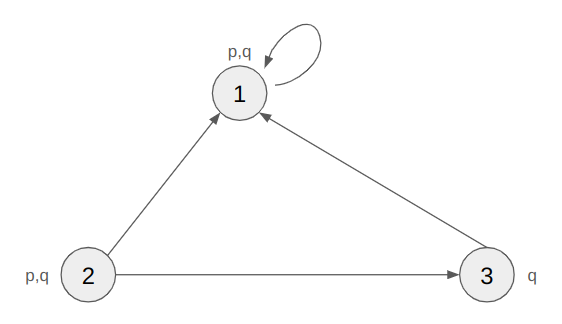
\includegraphics[width=0.75\textwidth]{images/maths/lmodal1.png}
    \caption{Un modelo $\mathcal{M}$.}
    \label{fig:lmodalimg1}
\end{figure}

Algunos ejemplos de fórmulas interesantes y su verdad sobre el modelo de la figura ~\ref{fig:lmodalimg1} son las siguientes:
\begin{itemize}
    \item $\square p $ es verdadera en los mundos (1,3). En 2 no lo es, porque para que lo sea, debería ser verdadera $p$ para todos los mundos a los que se puede acceder desde 2, y en el mundo 3 eso no ocurre.
    \item $\diamondsuit p$ es verdadera en todos los mundos (1,2,3).
    \item $\square q$ es verdadera en todos los mundos.
    \item $\diamondsuit q$ es verdadera en todos los mundos.
    \item $\square(p \rightarrow q)$ es verdadera en todos los mundos.
\end{itemize}

\subsection{Relaciones de consecuencia lógica}\label{subsection:lmodalconsec}
En la lógica modal, a diferencia de en la lógica proposicional, las consecuencias lógicas dependen de la estructura con la que se esté trabajando. Se definen las nociones de \textit{consecuencia local} y \textit{consecuencia global}.

\vspace{0.5cm}
\noindent
\textbf{Consecuencia local}

Sean $\phi$ una fórmula modal y $\Sigma$ un conjunto de fórmulas modales. Se dice que $\phi$ es \textbf{consecuencia local} de $\Sigma$, si para todo modelo $\mathcal{M} = \langle W,R,V \rangle$ y para todo $w \in W$ tal que para cada $\psi \in \Sigma$, $\psi$ es satisfacible en $w$, ocurre que $\phi$ es satisfacible en $w$. Cuando esto sucede, se escribe $\Sigma \models_l \phi$.

\vspace{0.5cm}
\noindent
\textbf{Consecuencia global}

Sean $\phi$ una fórmula modal y $\Sigma$ un conjunto de fórmulas modales. Se dice que $\phi$ es \textbf{consecuencia global} de $\Sigma$, si para todo modelo $\mathcal{M} = \langle W,R,V \rangle$ y para todo $w \in W$ tal que para cada $\psi \in \Sigma$, $\mathcal{M} \models \psi$, ocurre que $\mathcal{M} \models \phi$. Cuando esto sucede, se escribe $\Sigma \models_g \phi$.

\vspace{0.5cm}
Una particularidad de las definiciones anteriores, es que cuando $\Sigma = \emptyset$, entonces se tiene que ambas consecuencias son equivalentes, es decir, para toda fórmmula $\phi \in Form_{\mathcal{L}_{\mathcal{M}}}$:

\begin{align*}
    \models_l \phi \hspace{0.3cm} \Leftrightarrow \hspace{0.3cm} \models_g \phi
\end{align*}

\subsection{Sistemas lógicos modales}\label{subsection:lmodalsystems}
Dependiendo de las propiedades de la relación binaria escogida para los modelos $\mathcal{M}$, se tiene un sistema lógico formal modal diferente, es decir, se definen diferentes axiomatizaciones. Aquí se realiza una clasificación de algunas de las que existen, dependiendo de las condiciones del marco $\mathcal{F}$:

\begin{itemize}
    \item \textbf{K}: no hay condiciones en el marco.
    \item \textbf{D}: $R$ es serial.
    \item \textbf{T}: $R$ es reflexiva.
    \item \textbf{B}: $R$ es reflexiva y simétrica.
    \item \textbf{K4}: $R$ es transitiva.
    \item \textbf{S4}: $R$ es reflexiva y transitiva.
    \item \textbf{S5}: $R$ es reflexiva, simétrica y transitiva.
\end{itemize}

\subsection{Lógica modal y TLA}\label{subsection:lmodalTLA}
La relación de la Lógica Temporal de Acciones (TLA) que se presentará en la sección ~\ref{section:TLA} con la lógica modal, se manifiesta en cómo TLA incorpora y extiende los principios de la semántica de Kripke. En TLA, los ``mundos'' de la lógica modal se corresponden con ``estados'' en un sistema, y las ``relaciones de acceso'' se transforman en ``transiciones'' entre estos estados. Estas transiciones representan cambios o acciones en el sistema, permitiendo modelar el comportamiento dinámico de sistemas complejos a lo largo del tiempo.

Un aspecto clave a destacar es que la axiomatización considerada para TLA se basará en el sistema modal D, cuya relación de acceso es ``serial'', lo que significa que para cada mundo (o estado en TLA), existe al menos un mundo accesible (o estado siguiente). Esta característica es particularmente relevante en TLA, donde cada estado tiene un sucesor, reflejando la naturaleza continua y progresiva del tiempo y las acciones en sistemas dinámicos. 

En definitiva, en la siguiente sección se abordará con mayor rigor todos estos conceptos propios de TLA.

\section{Lógica Temporal de Acciones Proposicional (PTLA)}\label{section:TLA}
En esta sección se aborda el objetivo principal del capítulo: la Lógica Temporal de Acciones (TLA). Tras establecer las bases con la lógica proposicional, que simboliza el razonamiento humano en su forma más fundamental, se ha profundizado en la lógica modal, expandiendo el razonamiento a través de conceptos de \textit{necesidad} y \textit{posibilidad}. Esta extensión incluye la consideración de diversos mundos posibles, un aspecto esencial para entender la rica estructura de la TLA. Este marco conceptual sienta las bases para una comprensión integral de las lógicas temporales y se centra específicamente en la Lógica Temporal de Acciones, resaltando su capacidad para modelar dinámicas complejas a través de diferentes escenarios o ``mundos'', que serán nombrados como \textit{estados}.

La Lógica Temporal de Acciones fue definida por Leslie Lamport, en \cite{lamport1994temporal}, con el objetivo de verificar y especificar las propiedades de sistemas, particularmente concurrentes y distribuidos, mediante fórmulas. La motivación detrás de la definición de TLA por parte de Lamport radica en su convicción de que utilizar un razonamiento riguroso es la única manera de prevenir errores graves en algoritmo concurrentes. Esta percepción lleva al planteamiento de dos preguntas: ¿Por qué optar por una lógica en lugar de un lenguaje de programación convencional? ¿No sería más sencillo trabajar directamente con programas en lugar de fórmulas lógicas? La respuesta a ambas es no. ``\textit{La lógica es la formalización de las matemáticas de toda la vida, y las matemáticas de toda la vida son más simples que los programas}'', según comenta Lamport, no sin razón. Un lenguaje de programación puede usar términos matemáticos como \textit{función}, pero los constructos que representa no son tan simples como sus correspondientes conceptos matemáticos. Las funciones matemáticas son simples, mientras que en la mayoría de lenguajes de programación las funciones envuelven conceptos adicionales y complejos como \textit{expresión de retorno}, \textit{convención de llamada}, etc.

La naturaleza propia de la Lógica Temporal de Acciones está basada en la lógica de predicados, puesto que permite hacer razonamientos sobre estructuras complejas. Sin embargo, en esta sección se opta por presentar una axiomatización realizada por Martín Abadi \cite{abadi1990axiomatization}, usando para ello un enfoque proposicional de la TLA, denominada PTLA. Este enfoque proposicional representa una simplificación de TLA, reduciéndola a su forma más esencial y accesible. En PTLA, se utilizarán variables proposicionales en lugar de los términos más complejos de la lógica de predicados. Este enfoque es particularmente útil para introducir los conceptos fundamentales de las lógicas temporales sin la complejidad adicional de la lógica de predicados. En definitiva, el propósito es demostrar cómo los principios básicos de las lógicas temporales pueden ser utilizados para abordar y resolver problemas prácticos en el diseño y funcionamiento de sistemas informáticos, ofreciendo así una perspectiva valiosa sobre su aplicación práctica y relevancia en el mundo real.

\subsection{Modelos formales del tiempo}\label{subsection:TLAtime}
La Lógica Temporal de Acciones es \textbf{temporal} \cite{Pnueli1977TheTL}, \cite{gorankoRumberg2020temporal}. Eso quiere decir que los razonamientos realizados dependerán del \textbf{tiempo}. La primera cuestión a tratar es: ¿qué se entiende por \textit{tiempo}? ¿Qué ``tipo'' de tiempo se considera? La última pregunta se puede concretar y desglosar en otras varias: ¿Es un tiempo basado en \textit{intervalos} o en \textit{instantes}? ¿Es ese tiempo \textit{discreto}, \textit{denso}, o \textit{continuo}? ¿Hay \textit{principio}? ¿Y \textit{final}? Antes de poder hablar de PTLA, se muestran los dos tipos más básicos de modelos formales de tiempo, indicando al final cuál de los dos se escogerá para esta lógica particular.

\subsubsection{Modelos de tiempo basados en instantes}\label{subsubsection:TLAtimeinstant}
En estos modelos las entidades más primitivas son los \textbf{instantes de tiempo}, o también llamados \textbf{puntos en el tiempo}. Además, también se considera una relación binaria, escrita como $<$, para relacionar dichos puntos de tiempo. Por lo tanto, considerando $T$ como un conjunto no vacío de puntos temporales y $<$ una relación binaria sobre $T$, llamada \textbf{de precedencia}, el flujo temporal se puede representar como $\mathcal{T} = \langle T, <\rangle$. Esta relación de precedencia normalmente requiere que sea un \textbf{orden parcial}, esto es, es una relación irreflexiva, transitiva, y asimétrica (véase ~\ref{subsection:binaryrel}). 

Sin embargo, hay muchos modelos formales de tiempo basados en instantes. Los \textbf{modelos lineales} representan los instantes de tiempo como una linea, mientras que los \textbf{modelos lineales hacia atrás} permiten una representación ramificada, notando que el pasado es fijo (una linea), y el futuro es abierto (ramificándose en múltiples futuros posibles). Además, el ordenamiento temporal puede contener o no elementos mínimos o máximos, referentes al primer y último instante de tiempo, respectivamente.

Otra clasificación importante es la que se produce entre \textbf{modelos discretos}, \textbf{densos}, y \textbf{continuos}. Los modelos discretos \textit{hacia delante} indican que, cada instante de tiempo que tiene un sucesor, éste siempre tiene un sucesor inmediato correspondiente. En los modelos densos, por el contrario, entre dos instantes de tiempo subsiguientes cualesquiera, hay otro instante. Por otra parte, en los modelos continuos el orden temporal no sólo debe ser denso, sino que además, todo conjunto no vacío de instantes de tiempo que tiene un límite superior tiene un límite superior mínimo.

\subsubsection{Modelos de tiempo basados en intervalos}\label{subsubsection:TLAtimeinterval}
Este tipo de modelos aparecen cuando se necesita realizar razonamientos sobre eventos con duración. En este caso, las entidades primitivas son los \textbf{intervalos}. En estos modelos se presupone un tiempo lineal, aunque a diferencia de los modelos basados en instantes, aquí se pueden definir muchas más relaciones. Por todo ello, formalmente se define este flujo temporal como $\mathcal{T} = \langle T,<,\subset,O \rangle$, donde se tienen las relaciones binarias de precedencia $<$, inclusión $\subset$, y superposición $O$. No se entrará en más detalles acerca de este tipo de modelos.

\subsubsection{El modelo de tiempo de PTLA}\label{subsubsection:TLAtimedecision}
El modelo de tiempo considerado para la lógica temporal de acciones tendrá las siguientes características:
\begin{enumerate}
    \item \textbf{Basado en instantes}: En muchos sistemas, especialmente en informática y sistemas distribuidos, es crucial modelar y razonar sobre eventos en momentos específicos. Un modelo basado en instantes permite la representación precisa de cuándo ocurren acciones o cambios de estado. Este enfoque facilita el análisis preciso de secuencias de eventos y la sincronización entre acciones. Permite establecer relaciones causales y temporales claras entre eventos individuales.
    \item \textbf{Lineal}: Un modelo temporal lineal implica que para cualquier momento dado, hay un único ``futuro'' y un único ``pasado''. La linealidad simplifica el razonamiento sobre secuencias de eventos. Facilita la comprensión de las relaciones temporales, como ``antes'' y ``después'', y es más intuitiva para modelar muchos tipos de sistemas.
    \item \textbf{Discreto}: El tiempo se considera como un conjunto de momentos distintos y separados (por ejemplo, ``ticks'' de un reloj). Esto es particularmente adecuado para sistemas informáticos y digitales, donde las operaciones se realizan en pasos discretos.
    \item \textbf{Tiene un comienzo}: Siempre se considerará un punto de partida concreto: el \textit{instante 0}.
\end{enumerate}

\subsection{Estados. Comportamientos. Sistemas dinámicos}\label{subsection:TLAsystems}
El propósito de la Lógica Temporal de Acciones Proposicional es razonar sobre sistemas, especialmente concurrentes. Una aproximación unificada de programas secuenciales y concurrentes es lo que se denomina como \textit{sistema dinámico discreto}. Un \textbf{sistema dinámico discreto} $\mathcal{D}$ es un triple $\langle S, R, s_0 \rangle$ donde:

\begin{itemize}
    \item $S$ es el conjunto de estados del sistema (posiblemente infinito). Cada elemento, naturalmente, se denomina \textbf{estado}.
    \item $R$ es la relación de transición entre un estado y sus posibles sucesores. $R$ evidentemente, es una relación binaria que involucra sólo a dos estados.
    \item $s_0$ es el estado inicial.
\end{itemize}

En la sección ~\ref{subsec:concurrentatomic} ya se hizo una ligera mención a la noción de estados, transiciones entre ellos, y su relación con los programas concurrentes. Para dar una comprensión más detallada y clara apoyada en el concepto temporal, un estado en el contexto de un programa se puede visualizar como una ``instantánea'' en un punto específico del tiempo, denotado como $t = 0, 1, \ldots$. Esta instantánea captura y preserva todos los aspectos relevantes del sistema en ese momento, incluyendo los valores de sus variables y el estado de sus componentes internos. Cada estado, por lo tanto, refleja una configuración completa del sistema, proporcionando una base para entender y rastrear cómo y cuándo ocurren los cambios a lo largo del tiempo. 

Formalmente, se puede definir un estado como una función que asigna valores a todas las variables, donde una \textit{variable}  es un identificador que representa una propiedad específica o un atributo del sistema. Esta propiedad puede variar con el tiempo y es crucial para determinar el estado del sistema en cualquier momento dado. Las variables pueden representar una amplia gama de datos, como números, valores de verdad, o cadenas de texto, y son fundamentales para describir las características y el comportamiento del sistema. En otras palabras, $s$ por tanto queda determinada como:

\begin{align*}
    s : Var &\to Val \\
    x &\mapsto s(x)
\end{align*}

donde $Var$ y $Val$ denotan el conjunto de variables y de valores, respectivamente. El conjunto de valores puede contener diferentes tipos de elementos como números naturales, reales, e incluso cadenas de caracteres.

Por otra parte, un \textbf{comportamiento} o \textbf{ejecución} es una sucesión de estados (posiblemente infinita), escribiéndose:

\begin{align*}
    \sigma = \langle s_0, s_1, s_2, \ldots \rangle
\end{align*}

La relación de transición entre estados es no determinista en general (es decir, dado un estado $s$, su siguiente no tiene por qué ser siempre el mismo), por lo que diferentes secuencias de ejecución son posibles. Al conjunto de todos los posibles comportamientos de un sistema se escribe como $S^\infty$.

Para referirse al estado concreto de un comportamiento de un sistema, $\sigma \in S^\infty$, en un instante de tiempo $t$ concreto, se escribe $\sigma_t = s_t$. También, para referirse a la secuencia de estados que siguen al estado del sistema en el instante $t$, se escribe $\sigma^{+t} = \langle s_{t+1}, s_{t+2}, \ldots \rangle$. Se dice que un comportamiento $\sigma$ de un sistema está \textbf{detenido} cuando $\sigma_t = \sigma_0$, para todo instante de tiempo $t$. En caso contrario, se denota por $\mu(\sigma)$ como al primer instante de tiempo $t$ donde $\sigma_t \neq \sigma_0$.

\subsection{Acciones}\label{subsection:TLAactions}
La Lógica Temporal de Acciones basa sus principios en \textit{acciones}. En el contexto proposicional de esta lógica, una \textbf{acción} es un tipo especial de proposición que involucra al estado actual de una variable, y su estado siguiente. Un ejemplo de acción puede ser $A_0 := ``x' = x+1''$. $x$ es una variable que tiene un determinado valor actual, y $x'$ denota al estado de la variable en el instante de tiempo inmediatamente posterior. El operador $'$ juega un papel crucial en la definición sintáctica de PTLA, permitiendo formular afirmaciones sobre los estados futuros de las variables. En definitiva, la lectura de la acción puede hacerse como sigue: ``en el estado siguiente, el valor de $x$ será incrementado en una unidad con respecto a su valor actual''. 


\subsection{El lenguaje PTLA}\label{subsection:TLAlanguage}
Ahora, ya se puede hacer una definición formal del Lenguaje Proposicional Temporal de Acciones (PTA). Un \textbf{Lenguaje PTA} $\mathcal{L}_{TA}$ es una cuádrupla $(O,C,\mathcal{A},\mathcal{P})$ donde:

\begin{itemize}
    \item $O = \lbrace \neg, \land, \lor, \Rightarrow, \equiv \square, \diamondsuit \rbrace$ como el conjunto de conectivas u operadores lógicos. Aquí, el conjunto de conectivas primario considerado será $\lbrace \neg, \land, \lor \rbrace$, junto con los operadores modales $\lbrace \square, \diamondsuit \rbrace$
    \item $C = \lbrace \bot \rbrace$ es el conjunto de constantes proposicionales.
    \item $\mathcal{A}$ es el conjunto de \textbf{variables de acción}. Ejemplos son $A_0,A_1,A_2,\ldots$. Las variables de acción representan a proposiciones atómicas acerca de los estados de una variable, como se ha discutido en la sección anterior.
    \item $\mathcal{P}$ es el conjunto se variables proposicionales. Ejemplos son $P_0,P_1,P_2,\ldots$
\end{itemize}

Para poder trabajar con comodidad de aquí en adelante, se denomina \textbf{predicado de estado} a una combinación de los símbolos proposicionales con operadores lógicos, incluyendo también las constantes. Se escribirá como $Pred_{\mathcal{L}_{TA}}$ al conjunto de los predicados de estado del lenguaje. Si $P$ es un predicado de estado, se denota por $P'$ al \textbf{predicado de estado prima}, dando una afirmación sobre los componentes de $P$ pero en el estado inmediatamente posterior. Por otra parte, una \textbf{acción} será una combinación de predicados de estado, predicados de estado prima, y variables de acción, y se $Act_{\mathcal{L}_{TA}}$ es el conjunto de los acciones del lenguaje. Normalmente una acción se escribirá como $A,B,C, \ldots$.

Los términos de \textit{expresión},\textit{fórmula} y \textit{subfórmulas} siguen manteniendo las definiciones de la lógica proposicional y de la lógica modal. Sin embargo, ahora hay nuevas fórmulas a considerar. Son fórmulas de la lógica PTLA:

\begin{itemize}
    \item los predicados de estado.
    \item $[A]$, $\langle A \rangle \equiv \neg[\neg A]$, donde $A$ es una acción. El propósito de estas fórmulas quedará más claro cuando se introduzca su semántica.
    \item Si $F,G$ son fórmulas:
    \begin{itemize}
        \item $\neg F$, $F \land G$, $F \lor G$, son fórmulas.
        \item $\square F$, $\diamondsuit F \equiv \neg \square \neg F$, son fórmulas. A diferencia de en la lógica modal, ahora se leen ``siempre $F$'' y ``posible $F$'', respectivamente.
    \end{itemize}
\end{itemize}

Para poder entender mejor estas nuevas definiciones, se presenta un ejemplo. Sean $P_0,P_1$ variables proposicionales, y $A_0$ una variable de acción. Se definen las siguientes fórmulas:

\begin{itemize}
    \item $P_0 := x = 0$, y se lee como ``el valor de la variable $x$ es 0''.
    \item $P_1 := x = 1$, y se lee como ``el valor de la variable $x$ es 1''.
    \item A partir de $P_1$, se define $P_1' := x' = 1$, y se lee como ``el valor de la variable $x$ en el estado siguiente es 1''.
    \item $A_0 := x' = x+1$, y se lee como ``en el estado siguiente, el valor de la variable $x$ valdrá $1$ unidad más que el valor actual''. 

    \item $P_0 \land A_0 \Rightarrow P_1'$. Esto quiere decir que: ``Si el valor actual de $x$ es 0 ($P_0$) y ocurre la acción de incrementar $x$ en $1$, entonces en el estado siguiente el valor de $x$ será 1 $(P_1')$''.
\end{itemize}

La idea, introducida en ~\ref{subsection:lpropTLA}, es que las fórmulas TLA sirvan para especificar las propiedades de un programa concurrente, combinando el uso de predicados de estado con acciones que alteran los estados del sistema. Este enfoque resulta particularmente útil para la verificación de programas, donde las secuencias de eventos y las condiciones de sincronización son críticas.

\subsection{Semántica}\label{subsection:TLAsemantics}
El siguiente paso para poder determinar adecuadamente la lógica es dotar de significado a las fórmulas anteriormente descritas. La lógica modal es la que establece las bases para describir la semántica. En primer lugar, se entiende por \textbf{interpretación} al par $(S,I)$ donde:
\begin{itemize}
    \item $S$ es el \textit{espacio de estados}, conjunto no vacío ya introducido en la sección ~\ref{subsection:TLAsystems}, que contiene los posibles estados de un sistema dinámico discreto, como los programas.
    \item $I$ representa a un par de aplicaciones, $(I_\rho,I_\alpha)$ que asignan a cada variable proposicional $P_i, i \in \lbrace 0,1, \ldots \rbrace$ un subconjunto del espacio de estados $S$, y a cada variable de acción $A_i, i \in \lbrace 0,1, \ldots \rbrace$ un subconjunto de $S \times S$, respectivamente.
\end{itemize}

La idea intuitiva de los conjuntos que asignan las aplicaciones anteriores es la siguiente: $I_\rho(P_i)$ es el subconjunto de todos los estados donde $P_i$ es verdadera, noción estrechamente relacionada con lo introducido en ~\ref{subsection:lmodalsemantic}; mientras que  $I_\alpha(A_i)$ es el conjunto de pares de estados relacionados por $A_i$.

De manera análoga a lo que se realizó en ~\ref{subsection:lpropsemantic}, ahora se puede extender la definición de las funciones de interpretación para objetos sintácticos más complejos. Formalmente, las aplicaciones quedarían determinadas de la siguiente manera:

\begin{align*}
    I_\rho: Pred_{\mathcal{L}_{TA}} &\to S \\
    P &\mapsto I_\rho(P) \subset S
\end{align*}

\begin{align*}
    I_\alpha: Act_{\mathcal{L}_{TA}} &\to S \times S\\
    A &\mapsto I_\alpha(A) \subset S \times S
\end{align*}

\noindent
En el caso de los predicados de estado:

\begin{align*}
    I_\rho(\bot) &\triangleq \emptyset  \\
    I_\rho(\neg P) &\triangleq S \setminus I_\rho(P) \\
    I_\rho(P \land Q) &\triangleq I_\rho(P) \cap I_\rho(Q) \\
    I_\rho(P \lor Q) &\triangleq I_\rho(P) \cup I_\rho(Q)
\end{align*}

La forma de extender la interpretación a predicados de estado es bastante intuitiva. En el primer caso, la interpretación de la negación del predicado se relacionará con todos aquellos estados donde el predicado $P$ es falso, mientras que en el caso de la conjunción se contempla el conjunto de estados donde ambos predicados son verdaderos a la vez. Por otro lado, es evidente que para la conjunción de predicados de estado es suficiente con considerar la unión de los estados donde $P$ y $Q$ son verdad. Ahora, queda extender las interpretaciones a las acciones:


\begin{align*}
    I_\alpha(P) &\triangleq I_\rho(P) \times S \\
    I_\alpha(P') &\triangleq S \times I_\rho(P) \\
    I_\alpha(\neg A) &\triangleq (S \times S) \setminus I_\alpha(A) \\
    I_\alpha(A \land B) &\triangleq I_\alpha(A) \cap I_\alpha(B) \\
    I_\alpha(A \lor B) &\triangleq I_\alpha(A) \cup I_\alpha(B)
\end{align*}

La extensión de la función de interpretación a las acciones también es intuitiva. Lo primero que hay que recordar es que, los predicados de estado, también pueden ser considerados acciones. La interpretación de un predicado mediante $I_\alpha$ relaciona el subconjunto de espacios donde $P$ es verdadera con el espacio de estados completo. Esto significa que, desde cualquier estado donde $P$ es verdadero, la transición puede ir hacia cualquier otro estado del sistema, reflejando la idea de que la acción asociada a $P$ puede ocurrir en cualquier transición desde un estado donde $P$ es verdadero. En el caso de una acción que involucre al predicado de estado prima $P'$,  se considera la transición a estados donde $P$ será verdadero en el siguiente instante de tiempo, desde cualquier estado actual. Esto refleja la posibilidad de llegar a un estado donde $P$ es verdadero, partiendo de cualquier estado previo. En el caso de la negación de una acción, conjunción y disyunción de acciones el razonamiento es similar al dado para los predicados de estado.

\subsubsection{Modelos. Fórmulas satisfacibles y válidas}\label{subsubsection:TLAvalidForms}
Un \textbf{modelo} es un triple $\mathcal{M} =  \langle S,I,\sigma \rangle$, donde $(S,I)$ es una interpretación y $\sigma \in S^\infty$ es un comportamiento sobre $S$. La definición de \textbf{fórmula verdadera} en un modelo determinado se define inductivamente como sigue:

\begin{align*}
    \mathcal{M} \models P_j &\triangleq \sigma_0 \in I_\rho(P_j), \hspace{0.2cm} j \in \lbrace 0,1,\ldots \rbrace \\
    \mathcal{M} \models [A] &\triangleq \sigma \text{ está detenido ó } (\sigma_0,\sigma_{\mu(\sigma)}) \in I_\alpha(A) \\
    \mathcal{M} \models \bot &\triangleq \bot \\
    \mathcal{M} \models \neg F &\triangleq M \not \models F \\
    \mathcal{M} \models F \land G &\triangleq \mathcal{M} \models F \text{ y } \mathcal{M} \models G \\
    \mathcal{M} \models \square F &\triangleq \forall i \in \lbrace 0,1,2,\ldots \rbrace, \langle S,I,\sigma^{+i}\rangle \models F
\end{align*}

Se dice que $F$ es una \textbf{fórmula satisfacible} si existe un modelo $M = \langle S,I,\sigma \rangle$ de modo que $\mathcal{M} \models F$. Además, se dice que $F$ es una \textbf{fórmula válida} si $F$ es satisfacible para todo modelo $M$, y en ese caso, se escribe $\models F$.

\subsection{Axiomas de PTLA}\label{subsection:TLAaxioms}
Una lógica consta de una serie de axiomas que se asumen como verdaderas, y un conjunto de reglas que permiten hacer además algunas operaciones para deducir la veracidad de otras fórmulas del lenguaje. En este caso, Martín Abadi realizó una axiomatización de la Lógica Temporal de Acciones Proposicional, teniendo en cuenta una axiomatización basada en el sistema lógico D (ver ~\ref{subsection:lmodalsystems}). La lista de axiomas \footnote{El símbolo $\vdash$ se utiliza en la lógica para representar una relación de deducción o derivación. En el contexto de los sistemas lógicos, cuando se escribe $\vdash F$, significa que la fórmula $F$ es derivable o deducible a partir de un conjunto de axiomas y reglas de inferencia. En el caso de los axiomas, $\vdash$ se usa para enfatizar que se consideran verdaderos dentro del sistema lógico, formando la base de las derivaciones posteriores. No implica necesariamente que $F$ sea verdadera en un sentido absoluto, sino que es verdadera bajo las premisas y dentro del marco del sistema lógico aplicado.} es la siguiente:

\begin{enumerate}
    \item $ \vdash \square (F \Rightarrow G) \Rightarrow (\square F \Rightarrow \square G) $
    
    Este axioma indica la transmisión de la propiedad ``ser siempre verdadero'' a través de una implicación lógica.
    
    \item $ \vdash \square F \Rightarrow F $

    Este axioma refleja la idea de que la verdad perpetua de una fórmula, en particular lo es en el momento presente.
    
    \item $ \vdash \square F \Rightarrow \square\square F $

    Este axioma refuerza la idea de persistencia de verdad a través del tiempo.
    
    \item $ \vdash \square (\square F \Rightarrow G) \lor \square(\square G \Rightarrow F) $

    Este axioma es una manera clásica de expresar que el tiempo es lineal y que dos instantes cualesquiera en el futuro están ordenados. En el contexto del tiempo lineal sugiere que, en cualquier par de eventos en el tiempo, existe una relación de precedencia o causalidad entre ellos. Es decir, si un evento es perpetuo, esto afecta a la veracidad del otro, y viceversa.
    
    \item $ \vdash \square (\square(F \Rightarrow \square F)\Rightarrow F) \Rightarrow (\diamondsuit \square F \Rightarrow F) $

    Este axioma representa la naturaleza de que el tiempo es discreto. $\square(F \Rightarrow \square F)$ significa que siempre es cierto que si $F$ es verdadero, entonces $F$ será siempre verdadero en el futuro, indicando así una ``persistencia'' de $F$. Ahora, $\square (\square(F \Rightarrow \square F)\Rightarrow F)$ indica que si la persistencia futura de $F$ garantiza $F$, entonces $F$ debe ser cierta en el presente. Por otro lado $\diamondsuit \square F \Rightarrow F$ dice que si es posible que $F$ sea perpetuamente verdadera en el futuro, entonces $F$ es verdadera ahora. En esencia, la relación entre las dos partes establece que si la garantía de que una propiedad se mantendrá en el futuro significa que debe ser cierta ahora, entonces el hecho de que esa propiedad pueda ser perpetua en algún punto futuro también significa que debe ser cierta ahora.
    
    \item Si $\vdash F $ entonces $\vdash \square F $.

    Este axioma es un principio de generalización que indica que si una fórmula $F$ es verdadera, entonces siempre es verdadera.
    
    \item Si $ F $ es una instancia de una tautología proposicional entonces $\vdash \square F $.
    
    \item Si $ \vdash F $ y $ \vdash F \Rightarrow G $ entonces $ \vdash G $.

    Este axioma es un principio básico de la inferencia lógica.
    
    \item $ \vdash \lbrack \bot \rbrack \Rightarrow \lbrack A \rbrack $

    Este axioma maneja casos límite en la lógica de acciones. Si una acción imposible es verdadera, entonces cualquier acción $A$ es verdadera.
    
    \item $ \vdash \lbrack \bot \rbrack \Rightarrow \lbrack P \rbrack = P $

    Este axioma sirve para mantener la consistencia en el tratamiento de acciones imposibles.
    
    \item $ \vdash \lbrack \bot \rbrack \Rightarrow \lbrack \neg A \rbrack \equiv \neg \lbrack A \rbrack $

    Este axioma establece que bajo una acción imposible, la negación de una acción $A$ es equivalente a la negación de $A$ como una acción.
    
    \item $ \vdash \lbrack A \land B \rbrack \equiv \lbrack A \rbrack \land \lbrack B \rbrack $

    Este axioma indica la verdad de una acción definida por la conjunción de dos acciones.
    
    \item $ \vdash \lbrack (\neg P)' \rbrack \equiv \neg \lbrack P' \rbrack $

    \item $ \vdash \lbrack (P \land Q)' \rbrack \equiv \lbrack P' \rbrack \land \lbrack Q' \rbrack $
    \item $ \vdash \square P \Rightarrow \lbrack P' \rbrack $

    Este axioma indica que si un predicado $P$ es siempre verdadero, entonces la afirmación sobre $P$ en el estado siguiente ($P'$) también es verdadera.
    
    \item $ \vdash \square( P \Rightarrow ((\lbrack P' \rbrack \land G) \lor \square G )) \Rightarrow (([P'] \land G) \Rightarrow \square G)$

    Este axioma se puede ver como sigue: supongamos que siempre que $P$ sea verdadero, entonces o bien $G$ es verdadero y $P$ sobrevive al siguiente cambio de estado, o $G$ es verdadero para siempre. Esto implica que $G$ se mantiene verdadero mientras $P$ se mantiene verdadero, y se vuelve verdadero para siempre si $P$ deja de ser verdadero. Por lo tanto, si $G$ es verdadero inicialmente y $P$ es verdadero después del primer cambio de estado, entonces $G$ es siempre verdadero. 
    
    En definitiva es útil para modelar situación donde la verdad de una condición o propiedad depende de la persistencia de otra a lo largo del tiempo. Por ejemplo, en sistemas de software, podría utilizarse para modelar cómo diversas condiciones deben mantenerse mientras otras condiciones sigan siendo verdaderas.
\end{enumerate}

\subsubsection{Algunas consecuencias de los axiomas}\label{subsubsection:TLAconseq}
Algunas consecuencias de los axiomas presentados para la lógica temporal de acciones proposicional son las citadas a continuación:

\begin{enumerate}
    \item $\vdash [\bot] \Rightarrow (F \equiv \square F) \land (F \equiv \diamondsuit F)$

    Esta fórmula indica que, una vez se ha detenido la ejecución, todas las características permanecen permanentes, significando que $F$,$\square F$ y $\diamondsuit F$ son equivalentes, para toda $F$.
    
    \item $\vdash \langle P' \rangle \Rightarrow \diamondsuit P$

    En palabras, si la ejecución no se ha detenido y la siguiente acción es P', entonces P eventualmente sucederá. Esta fórmula indica una forma sencilla de probar propiedades de vivacidad.

    
    \item $\vdash P \land \square(P \Rightarrow [P']) \Rightarrow \square P$

    Esta fórmula es una consecuencia de instanciar $G$ por $P$ en el Axioma 16.
    
    \item $\vdash [P'] \land \diamondsuit G \Rightarrow G \lor \diamondsuit (P \land \diamondsuit G)$

    Este teorema es una consecuencia del Axioma 16. Dice que si la acción $P'$ va a tener lugar (siempre que la ejecución no se haya detenido) y $G$ debe darse eventualmente, entonces o $G$ es verdadera ahora, o $P$ sucederá eventualmente y $G$ sucederá más tarde.
    
    \item $\vdash (P \land \diamondsuit G \land \square (P \land \diamondsuit G \Rightarrow [P'])) \Rightarrow \diamondsuit (P \land G)$

    Esta fórmula es el dual del Axioma 16. En otras palabras, mientras que el Axioma 16 se enfoca en la persistencia de una condición y su impacto en otra, esta fórmula considera las condiciones necesarias para que dos propiedades se cumplan eventualmente en el futuro.
\end{enumerate}

\subsection{Solvencia y complitud}\label{subsection:TLAcompleteness}
En el estudio de cualquier sistema lógico, dos propiedades fundamentales a considerar son la solvencia (o corrección) y la completitud. Estos conceptos son cruciales para evaluar la robustez y confiabilidad del sistema lógico, especialmente en un contexto como el de PTLA, donde se trata de capturar y razonar sobre el comportamiento de sistemas concurrentes y distribuidos.

La \textbf{solvencia} de un sistema lógico se refiere a la garantía de que todas las fórmulas que pueden ser deducidas dentro del sistema son verdaderas en todos los modelos del sistema. En el contexto de PTLA, esto significa que si una fórmula $F$ puede ser deducida $\vdash F $, entonces $F$ debe ser verdadera en cada modelo de PTLA $ \mathcal{M} \models F $ para todo modelo $\mathcal{M}$. La solvencia asegura que el sistema no permite derivar conclusiones falsas o inconsistentes a partir de sus axiomas y reglas de inferencia.

La \textbf{completitud}, por otro lado, se refiere a la capacidad del sistema lógico para derivar todas las fórmulas verdaderas en todos los modelos. En PTLA, un sistema es completo si, para cada fórmula $ F $ que es verdadera en todo modelo $ \mathcal{M} \models F $ para todo modelo $ \mathcal{M} $, existe una derivación de $ F $ dentro del sistema $ \vdash F $. La completitud asegura que el sistema es capaz de capturar todas las verdades que se pueden expresar en su lenguaje.

En la Lógica Temporal de Acciones Proposicional, se verifican dos teoremas fundamentales relacionados con estos conceptos:

\begin{teorema}
    Sea $G$ una fórmula. Si $G$ no es deducible, entonces $\neg G$ tiene un modelo.
\end{teorema}

\begin{teorema}
    \textbf{Solvencia y complitud}: Sea $F$ una fórmula. $\vdash F \Leftrightarrow \hspace{0.1cm} \models F$.
\end{teorema}

\subsection{Ejemplo práctico de especificación con PTLA}\label{subsection:PTLAExample}
Para poder en valor todo el estudio matemático realizado a lo largo de este capítulo, se ofrecerá un ejemplo muy sencillo de cómo la Lógica Temporal de Acciones puede ayudar a la especificación de programas, entre ellos los concurrentes, que son el objeto de estudio global de todo el proyecto tanto teóricamente como en la práctica.

El siguiente ejemplo denota un simple programa que cuando se ejecuta, permanece incrementando las dos únicas variables que posee $x,y$ inicializadas a 0, eligiendo de forma no determinística cuál incrementar.

\begin{figure}[ht]
\centering
\begin{lstlisting}[basicstyle=\ttfamily\small, frame=single]
    var natural x,y = 0;
    do 
       < true -> x := x + 1 >
       [ ]
       < true -> y := y + 1 >
    od
\end{lstlisting}
\caption{Ejemplo de programa para especificación: Incremento.}
\label{fig:TLAincrement}
\end{figure}

\begin{figure}[h]
    \centering
    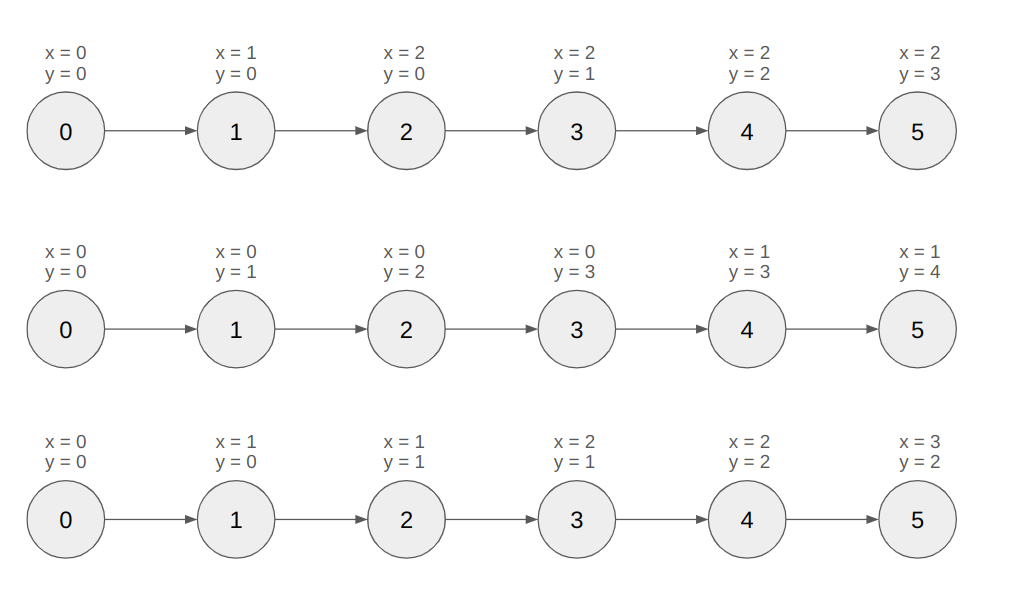
\includegraphics[width=0.9\textwidth]{images/maths/ptla1.png}
    \caption{Diferentes comportamientos del programa Incremento.}
    \label{fig:TLAincrementBehav}
\end{figure}

La figura ~\ref{fig:TLAincrementBehav} culmina todos los conceptos tratados hasta el momento en este capítulo. En primer lugar, se dispone de un conjunto posiblemente infinito de estados $S$, que están representados por los nodos o círculos azules, y que indican el valor de las variables en un instante de tiempo $t$ determinado, esto es, en el estado 0 se indica el valor de las variables en el instante 0, y así sucesivamente. Además, desde el punto de vista de la lógica modal, se puede ver a $S$ como el conjunto de todos los mundos posibles, y su relación entre ellos, que es de tipo serial, pues cada estado (o ``mundo'') tiene al menos un estado sucesor (o ``mundo accesible''), en consonancia con lo mencionado en la axiomatización de PTLA. Para finalizar, se refleja la propiedad de no determinismo de dicha relación, pues aunque siempre se relacione el estado $s_1$ con $s_2$, su naturaleza en las tres diferentes secuencias no es la misma, debido al funcionamiento intrínseco del programa de elegir indiscriminadamente qué variable incrementar, propiciando diferentes comportamientos.

En primer lugar, se recuerda que en ~\ref{subsection:TLAtime} se definió el modelo temporal sobre el que se sustenta el razonamiento sobre los sistemas concurrentes. $\mathcal{T} = \langle T, < \rangle$ es el modelo formal elegido donde $<$ es un orden parcial. Los instantes de tiempo de ejecución del programa empiezan en el segundo $0$, evolucionando discreta y linealmente. A continuación, se puede denotar por $\mathcal{D} = \langle S, R, s_0 \rangle$ al sistema dinámico que representa el programa de incremento, donde $R$ es una relación binaria serial, pues partiendo de un estado concreto, siempre se puede acceder a otro estado siguiente. En la figura ~\ref{fig:TLAincrementBehav} se representan tres comportamientos diferentes del programa: $\sigma_0, \sigma_1, \sigma_2 \in S^\infty$, respectivamente.

Se llamará $\Phi$ a la fórmula que especificará el programa al completo. En primer lugar, se puede especificar el estado inicial del programa utilizando las siguientes proposiciones y construyendo la fórmula (concretamente el predicado de estado) $Init_{\Phi}$:

\begin{align*}
    P_0 &\triangleq x = 0 \\
    P_1 &\triangleq y = 0 \\
    Init_{\Phi} &\triangleq P_0 \land P_1
\end{align*}

\noindent
Lo que deja a la fórmula $\Phi$ por el momento como:

\begin{align*}
    \Phi \triangleq Init_{\Phi}
\end{align*}

A continuación, por las características del programa se pueden tomar dos diferentes \textit{acciones}: o incrementar en una unidad la variable $x$, o hacer lo propio con la variable $y$. Esto se puede escribir de la siguiente manera:

\begin{align*}
    A_0 &\triangleq x' = x+1 \hspace{0.3cm} &\text{(Incrementar x)} \\
    A_1 &\triangleq y' = y \hspace{0.3cm} &\text{(Dejar sin cambios y)}\\
    A_2 &\triangleq x' = x \hspace{0.3cm} &\text{(Dejar sin cambios x)} \\
    A_3 &\triangleq y' = y+1 \hspace{0.3cm} &\text{(Incrementar y)} \\
    A &\triangleq A_0 \land A_1 \hspace{0.3cm} &\text{(Incrementar x, no modificar y)} \\
    B &\triangleq A_2 \land A_3 \hspace{0.3cm} &\text{(No modificar x, incrementar y)} \\
    \mathcal{A} &\triangleq A \lor B \hspace{0.3cm} &\text{(Ocurre la acción A u ocurre la acción B)}
\end{align*}

Ahora, se puede actualizar la fórmula $\Phi$ que especifica al programa añadiendo la siguiente fórmula:

\begin{align*}
    \Phi \triangleq Init_{\Phi} \land [\mathcal{A}]
\end{align*}

Con esto, lo que estamos diciendo es que, para cualquier punto en el comportamiento del programa después de $Init_{\Phi}$ , si el programa no se ha detenido, entonces la acción que sigue es o incrementar $x$ (acción $A$) o incrementar $y$ (acción $B$), y estas son las únicas transiciones posibles. La fórmula $\Phi$ tiene modelos que la satisfacen, concretamente:

\begin{align*}
    \langle S, I, \sigma_i \rangle \models \Phi, \hspace{0.3cm} i \in \lbrace 0,1,2 \rbrace
\end{align*}

En particular, es algo que siempre ocurre en todos los estados a partir del estado inicial (siempre que el programa no se haya detenido). En otras palabras, es una fórmula que se satisface para todo modelo considerado, por lo que se puede escribir la fórmula:

\begin{align*}
    \Phi \triangleq Init_{\Phi} \land \square[\mathcal{A}]
\end{align*}

Así, se indica que la ejecución de la acción se satisface en todos los subsiguientes estados después del inicio, sin excepción. La fórmula $\Phi$ ya presenta una propiedad para el programa, concretamente la \textit{propiedad de seguridad}, garantizando que nunca ocurrirán otras acciones no especificadas, lo que podría ser considerado como un ``comportamiento malo''. En otras palabras, el programa está restringido a comportarse de manera segura tal como se ha definido por las acciones.

\textbf{Otros sistemas lógicos para verificación de sistemas}\label{section:otherlogics}
La Lógica Temporal de Acciones en definitiva es un excelente sistema lógico formal para razonar sobre las propiedades de los sistemas concurrentes. Sin embargo, no es el único sistema lógico formal que se utiliza, sino que hay una gran variedad de ellos que pueden ser utilizados para ese mismo fin. A continuación, se mencionan brevemente comparando sus enfoques con el de TLA:

\begin{itemize}
    \item \textbf{Lógica Temporal Lineal (LTL)}:
    \begin{itemize}
        \item \textit{Enfoque}: Se centra en el comportamiento de los sistemas a lo largo del tiempo, permitiendo hacer afirmaciones sobre secuencias de estados en el futuro.
        \item \textit{Comparación con TLA}: TLA se orienta hacia acciones y transiciones entre estados, mientras que LTL se enfoca en las propiedades de los estados a lo largo del tiempo.
    \end{itemize}
    
    \item \textbf{Lógica Temporal de Árbol Computacional (CTL)}:
    \begin{itemize}
        \item \textit{Enfoque}: Permite expresar propiedades sobre árboles de ejecución, representando múltiples futuros posibles desde un mismo estado.
        \item \textit{Comparación con TLA}: CTL es más adecuada para sistemas no deterministas con varias posibilidades de evolución, a diferencia de TLA que es más lineal.
    \end{itemize}
    
    \item \textbf{Lógica de Hoare \footnote{En particular, este sistema lógico formal es el que se enseña en la asignatura de \textit{Sistemas Concurrentes y Distribuidos}.}}: 
    \begin{itemize}
        \item \textit{Enfoque}: Se centra en la corrección de programas individuales mediante tripletas que relacionan estados iniciales y finales con una instrucción. 
        \item \textit{Comparación con TLA}: Mientras la Lógica de Hoare es más adecuada para programas secuenciales, TLA es más efectiva en sistemas concurrentes y distribuidos.
    \end{itemize}
    
    \item \textbf{Lógica de Separación (Separation Logic)}:
    \begin{itemize}
        \item \textit{Enfoque}: Utilizada para razonar sobre programas que manipulan estructuras de datos mutables en memoria.
        \item \textit{Comparación con TLA}: Es específica para estructuras de datos y manejo de memoria, mientras que TLA tiene una aplicación más general.
    \end{itemize}
\end{itemize}

